\section{Conjunto de datos}

Según la revisión de Pandey et al. \cite{PANDEY2021114595}, en la investigación sobre SFP se ha utilizado una gran variedad de conjuntos de datos. Su evidencia empírica muestra que el conjunto de datos de la NASA es el más aplicado en la disciplina, seguido de los conjuntos de datos de código abierto y del repositorio PROMISE.


\begin{figure}[H]
    \centering
    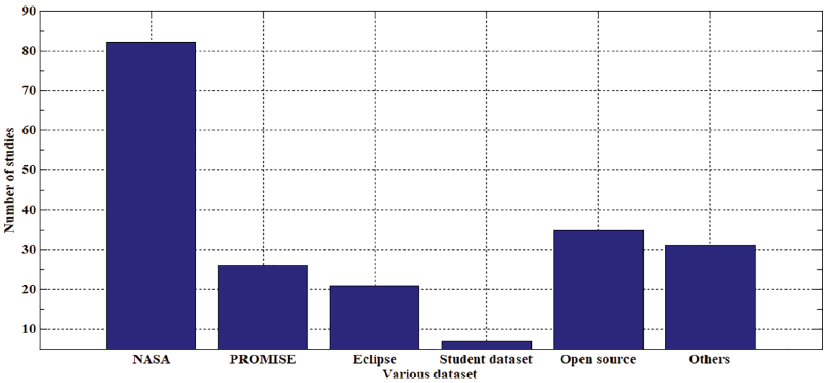
\includegraphics[width=\textwidth]{chapters/ChapterMarcoTeorico/sections/Datasets/fig/SFP dataset.png}
    \setstretch{1} %Interlineado 1
	\captionsetup{labelsep=period, labelfont=bf}
    \caption{Porcentaje de estudios para diferentes conjuntos de datos que se utilizan en SFP. \cite{PANDEY2021114595}}
    \label{fig:SFPDataset}
\end{figure}

Se pueden encontrar algunos patrones en la Figura \ref{fig:datasetdist} en que el conjunto de datos con la distribución de fallos más baja es popularmente utilizado y viceversa. Según el gráfico de barras, los conjuntos de datos de la NASA tienen menos distribución de fallos (CM1, PC1, KC3, MW1, PC4) en comparación con el conjunto de datos del repositorio PROMISE (poi-3.0, lucene-2.4, eclipse-3.0, eclipse-2.1). Una información adicional que informa esta figura es que, en algunos casos, los conjuntos de datos que tienen un gran número de instancias tienen menos distribución de fallos, como JM1. CM1 y JM1 también son conjuntos de datos sustancialmente utilizados que combinan el 57\% de los estudios y contienen el 31\% de los módulos defectuosos.

\begin{figure}[H]
    \centering
    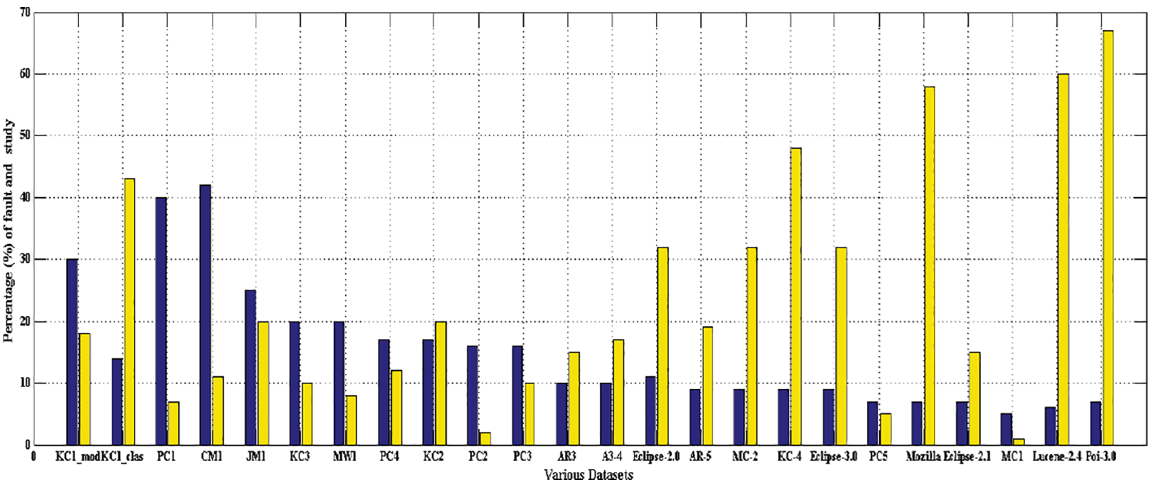
\includegraphics[width=\textwidth]{chapters/ChapterMarcoTeorico/sections/Datasets/fig/datasetdist.png}
    \setstretch{1} %Interlineado 1
	\captionsetup{labelsep=period, labelfont=bf}
    \caption{Distribución de errores de diferentes conjuntos de datos. \cite{PANDEY2021114595}}
    \label{fig:datasetdist}
\end{figure}